\documentclass{article}


\usepackage{arxiv}

\usepackage[utf8]{inputenc} % allow utf-8 input
\usepackage[T1]{fontenc}    % use 8-bit T1 fonts
\usepackage{hyperref}       % hyperlinks
\usepackage{url}            % simple URL typesetting
\usepackage{booktabs}       % professional-quality tables
\usepackage{amsfonts}       % blackboard math symbols
\usepackage{nicefrac}       % compact symbols for 1/2, etc.
\usepackage{microtype}      % microtypography
\usepackage{lipsum}
\usepackage{threeparttable}
\usepackage{multicol}
\usepackage{multirow}
\usepackage{setspace}
\usepackage{pdfpages}
\usepackage{algpseudocode}  
\usepackage{algorithm}  
\usepackage{amsmath}  
\usepackage{float}
\usepackage{subfigure} 
\usepackage{array}
\usepackage{longtable}
\usepackage{rotating}
\usepackage{diagbox}

\title{Multimodal Machine Translation}

\author{Feiyang Chen}

% \author{
%   David S.~Hippocampus\thanks{Use footnote for providing further
%     information about author (webpage, alternative
%     address)---\emph{not} for acknowledging funding agencies.} \\
%   Department of Computer Science\\
%   Cranberry-Lemon University\\
%   Pittsburgh, PA 15213 \\
%   \texttt{hippo@cs.cranberry-lemon.edu} \\
%   %% examples of more authors
%   \And
%  Elias D.~Striatum \\
%   Department of Electrical Engineering\\
%   Mount-Sheikh University\\
%   Santa Narimana, Levand \\
%   \texttt{stariate@ee.mount-sheikh.edu} \\
%   %% \AND
%   %% Coauthor \\
%   %% Affiliation \\
%   %% Address \\
%   %% \texttt{email} \\
%   %% \And
%   %% Coauthor \\
%   %% Affiliation \\
%   %% Address \\
%   %% \texttt{email} \\
%   %% \And
%   %% Coauthor \\
%   %% Affiliation \\
%   %% Address \\
%   %% \texttt{email} \\
% }

\begin{document}
\maketitle

% \begin{abstract}
% \lipsum[1]
% \end{abstract}


% keywords can be removed
% \keywords{First keyword \and Second keyword \and More}


\section{Task: Video-guided Machine Translation}

The multimodal machine translation task aims at generating a better target sentence by supplementing the source sentence with extra information gleaned from other modalities. Previous studies mainly focus on using images as the visual modality to help machine translation \cite{specia2016shared,elliott2017findings,barrault2018findings}. Video-guided Machine Translation (VMT) was first proposed by (Wang et al., 2019) \cite{wang2019vatex} to translate a source language sentence into the target language using the video information as additional spatiotemporal context. They designed a multimodal Seq2Seq model with the attention mechanism for VMT, which the overview is shown in Figure \ref{Fig.main}, including three modules: 1). Source Encoder; 2). Video Encoder; and 3). Target Decoder. 


	\begin{figure*}[htbp] 
		\centering
		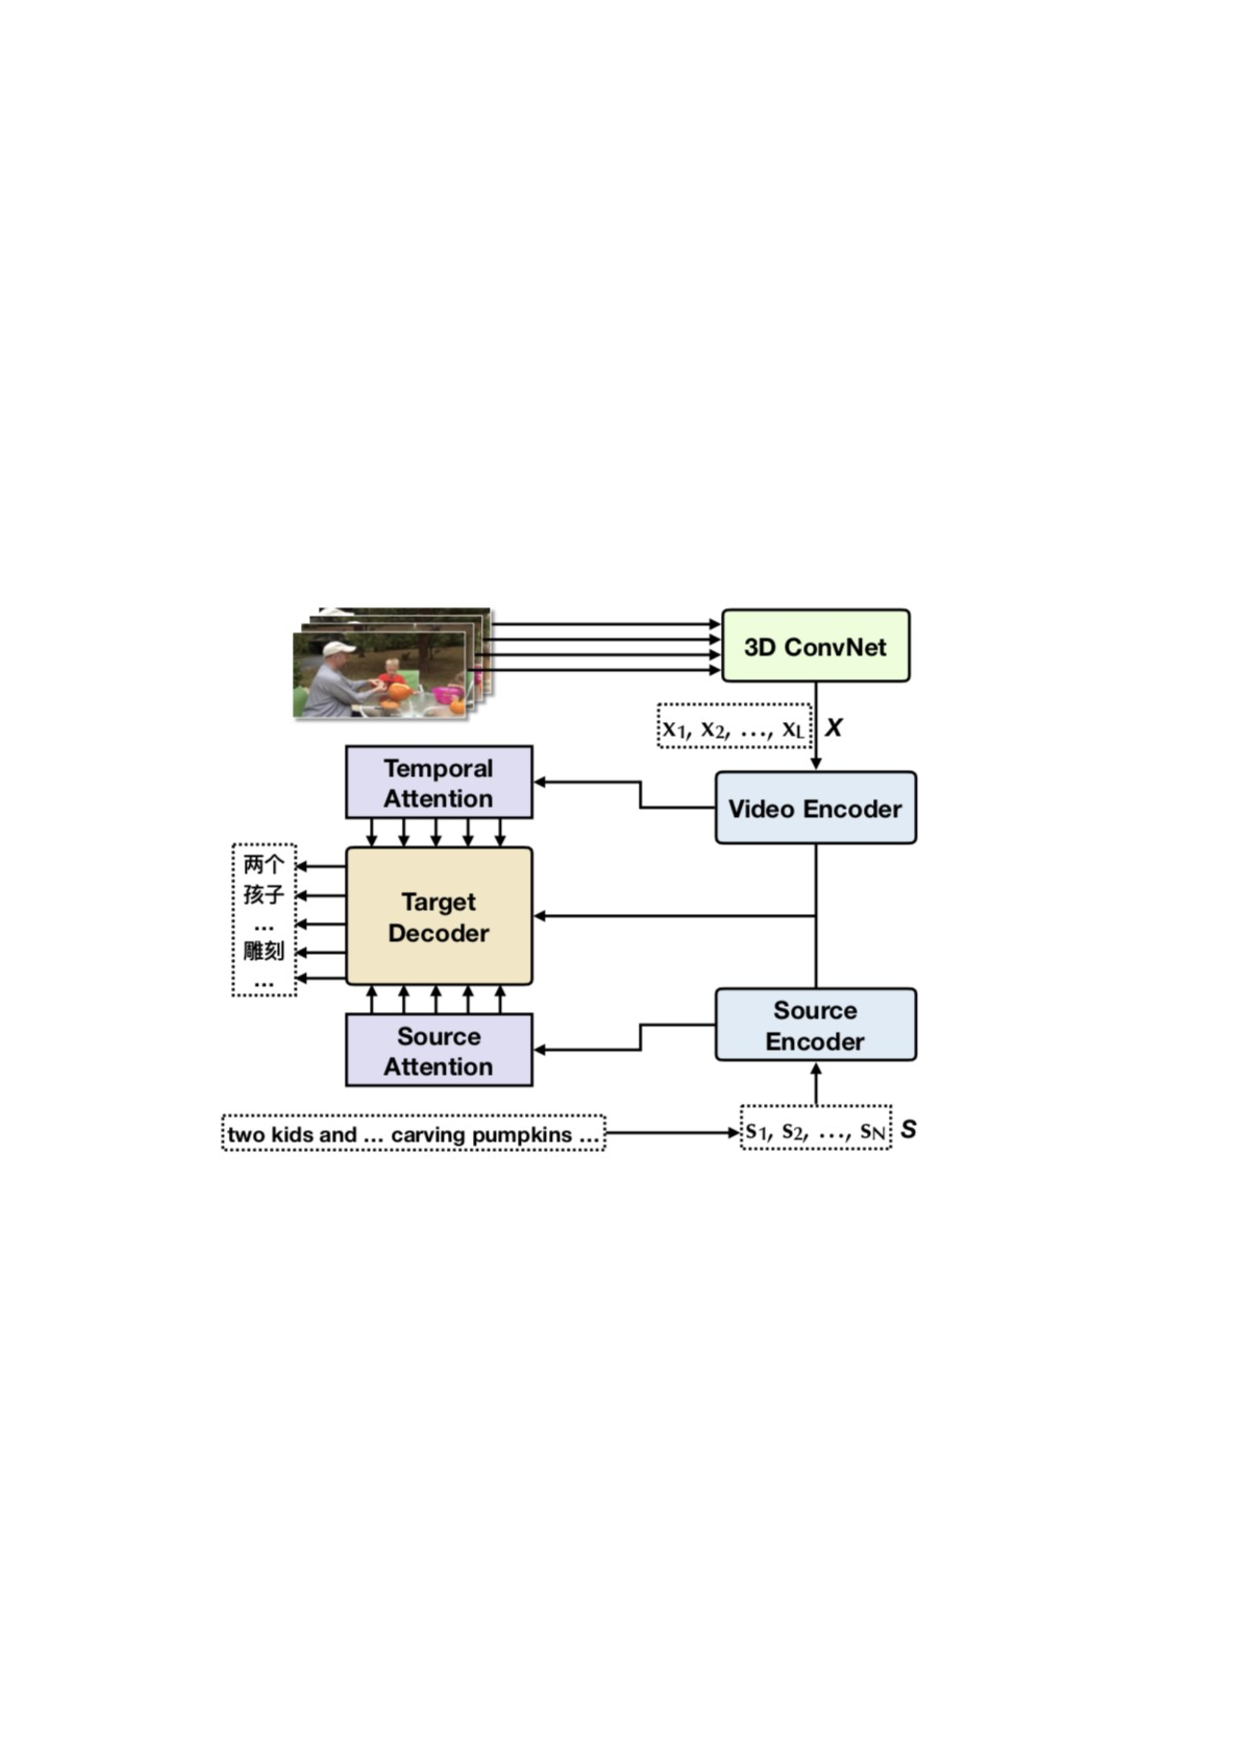
\includegraphics[width=0.5\textwidth]{baseline.pdf} 
		\caption{Video-guided machine translation model from (Wang et al., 2019) \cite{wang2019vatex}.}
		\label{Fig.main} 
	\end{figure*}
	
	
	\begin{figure*}[htbp] 
		\centering
		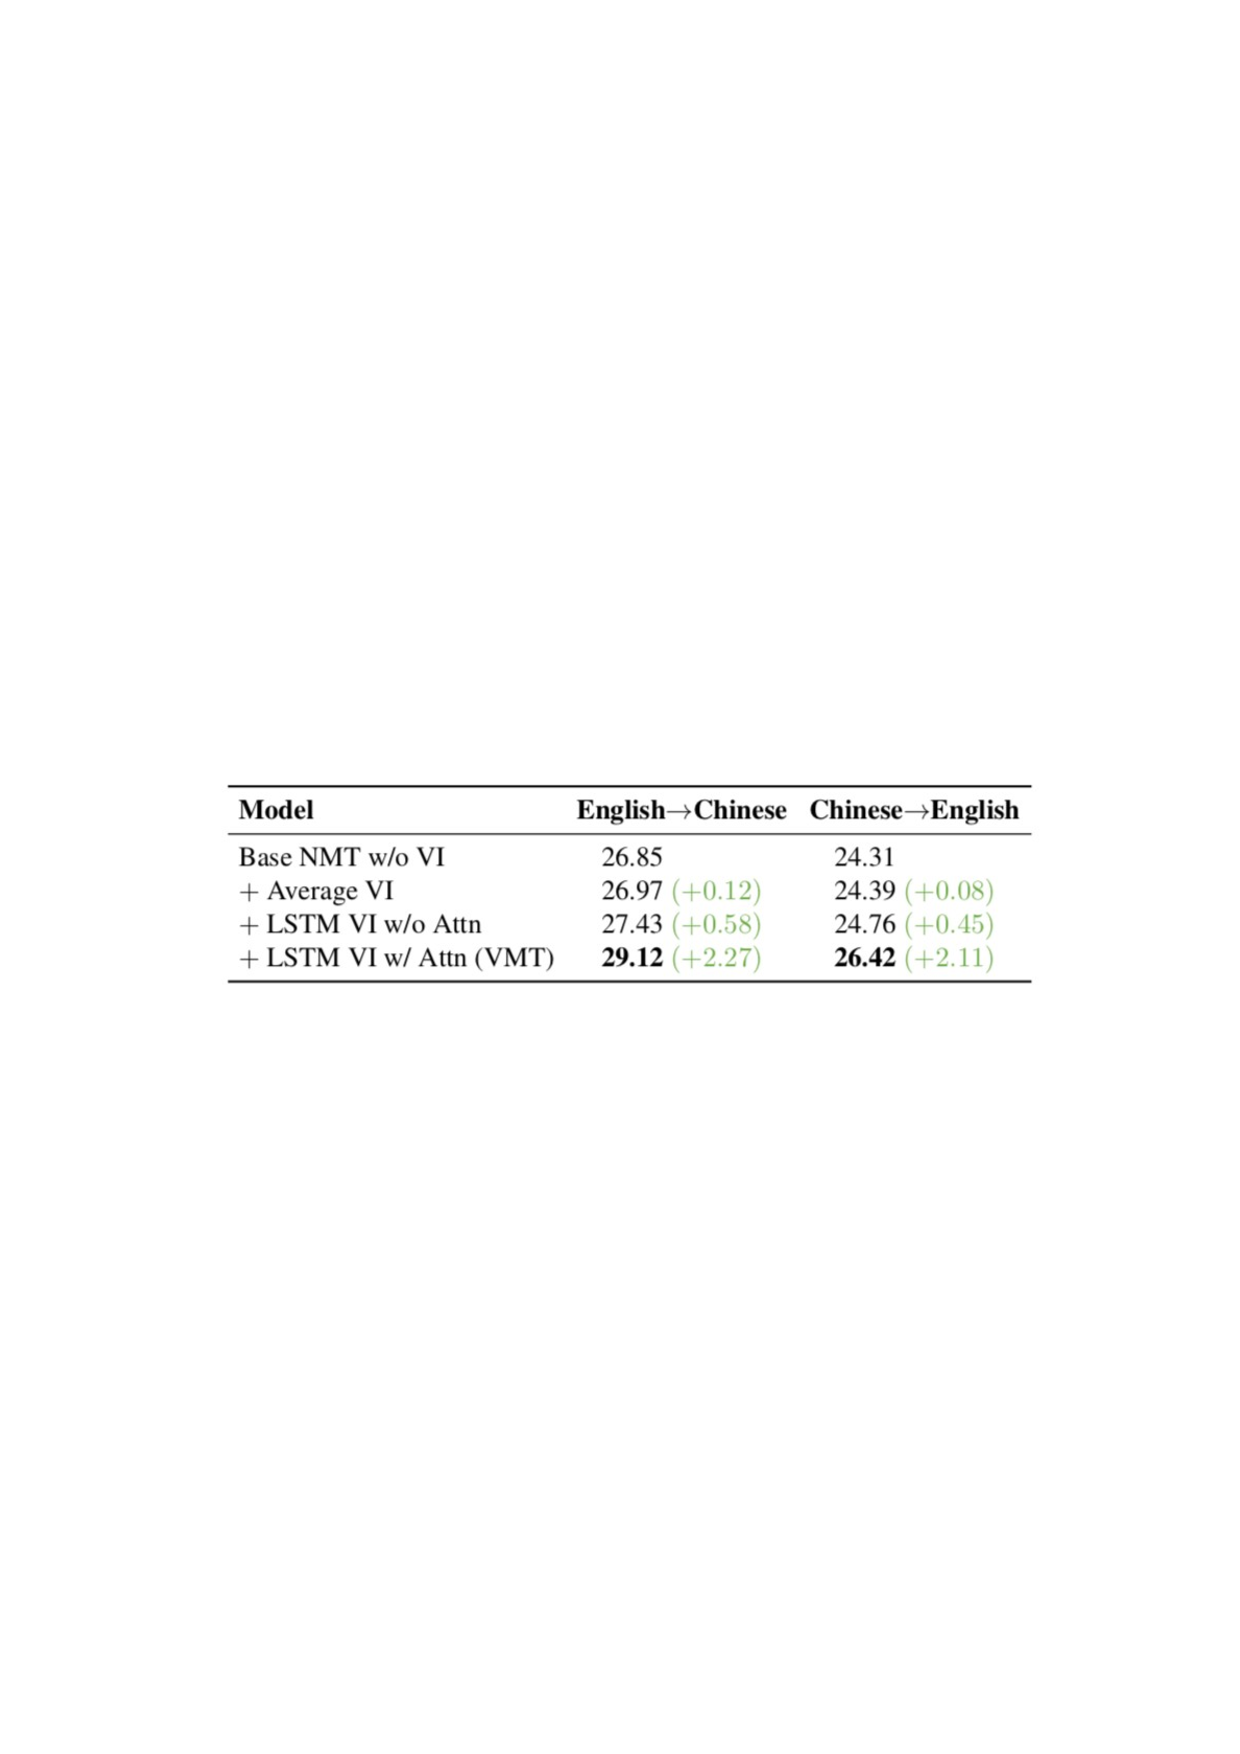
\includegraphics[width=0.7\textwidth]{results.pdf} 
		\caption{Experimental results from (Wang et al., 2019) \cite{wang2019vatex}, which are reported on the BLEU-4 scores. VI: video features from the pretrained I3D model. Attn: temporal attention mechanism.}
		\label{Fig.main2} 
	\end{figure*}
	
	
However, they do not have an in-depth analysis of why video information can better help machine translation. According to their experimental results, the marginal improvements by the Average video Features and the LSTM Video Features reveal that passively receiving and incorporating the video features is ineffective in helping align source and target languages, only improvement within \%1 range, as is shown in Figure \ref{Fig.main2}. At the same time, they observe that the translation system achieves much better performance when using the LSTM Video Features with temporal attention (the full VMT model) to dynamically interact with the video features. They explained it as because with the attention mechanism, the language dynamics are used as a query to highlight the relevant spatiotemporal features in the video, and then the learned video context would assist the word mapping between source and target language spaces. But in what ways does the video-level features help the machine translation? Is it just to help ordinary text machine translation to disambiguate?



\section{Ideas}

\subsection{Representation Learning}

Inspired by (Tan et al., 2019) \cite{tan2019lxmert}, as is shown in Figure \ref{Fig.main3}, we can study how the temporal and spatial information from Video and Text modality interact to improve machine translation performance. Consider a series of probing experiments to explore deeper into how video-level features to help machine translation.


	\begin{figure*}[htbp] 
		\centering
		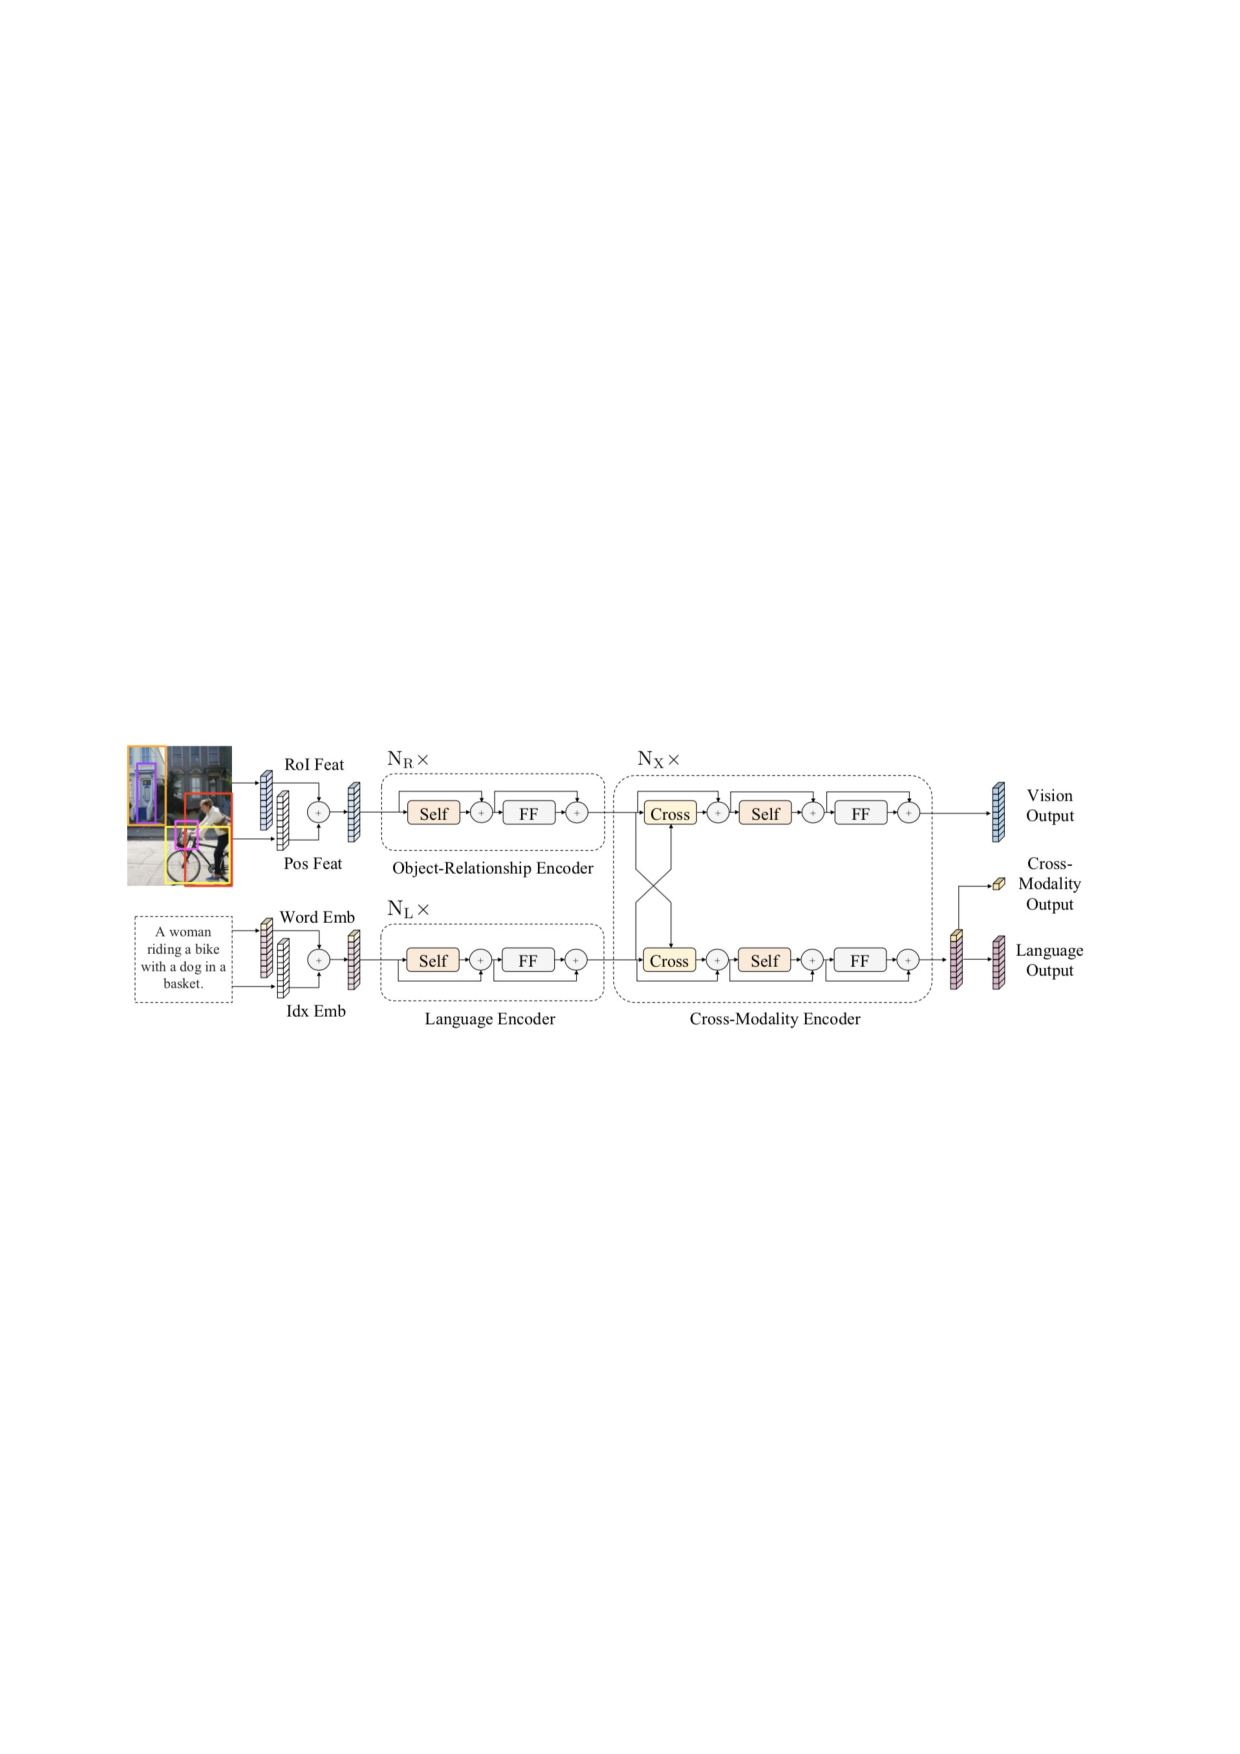
\includegraphics[width=0.8\textwidth]{LXMERT.pdf} 
		\caption{The LXMERT model from (Tan et al., 2019) \cite{tan2019lxmert} for learning vision-and-language cross-modality representations. ‘Self’ and ‘Cross’ are abbreviations for self-attention sub-layers and cross-attention sub-layers, respectively. ‘FF’ denotes a feed-forward sub-layer.}
		\label{Fig.main3} 
	\end{figure*}


\subsection{Multi-Task Learning}

(Pramanik et al., 2019) \cite{pramanik2019omninet} proposed a spatio-temporal cache mechanism that enables learning spatial dimension of the input in addition to the hidden states corresponding to the temporal input sequence, as is shown in Figure \ref{Fig.main4}. The proposed architecture further enables a single model to support tasks with multiple input modalities as well as asynchronous multi-task learning. Accordingly, we can consider machine translation as the target task learning. When Video-guided Machine Translation task and  Multilingual Video Captioning task combine to mutual learning, we are expected to solve some challenges that exist in current machine translation, such as Zero-resource Translation.


	\begin{figure*}[htbp] 
		\centering
		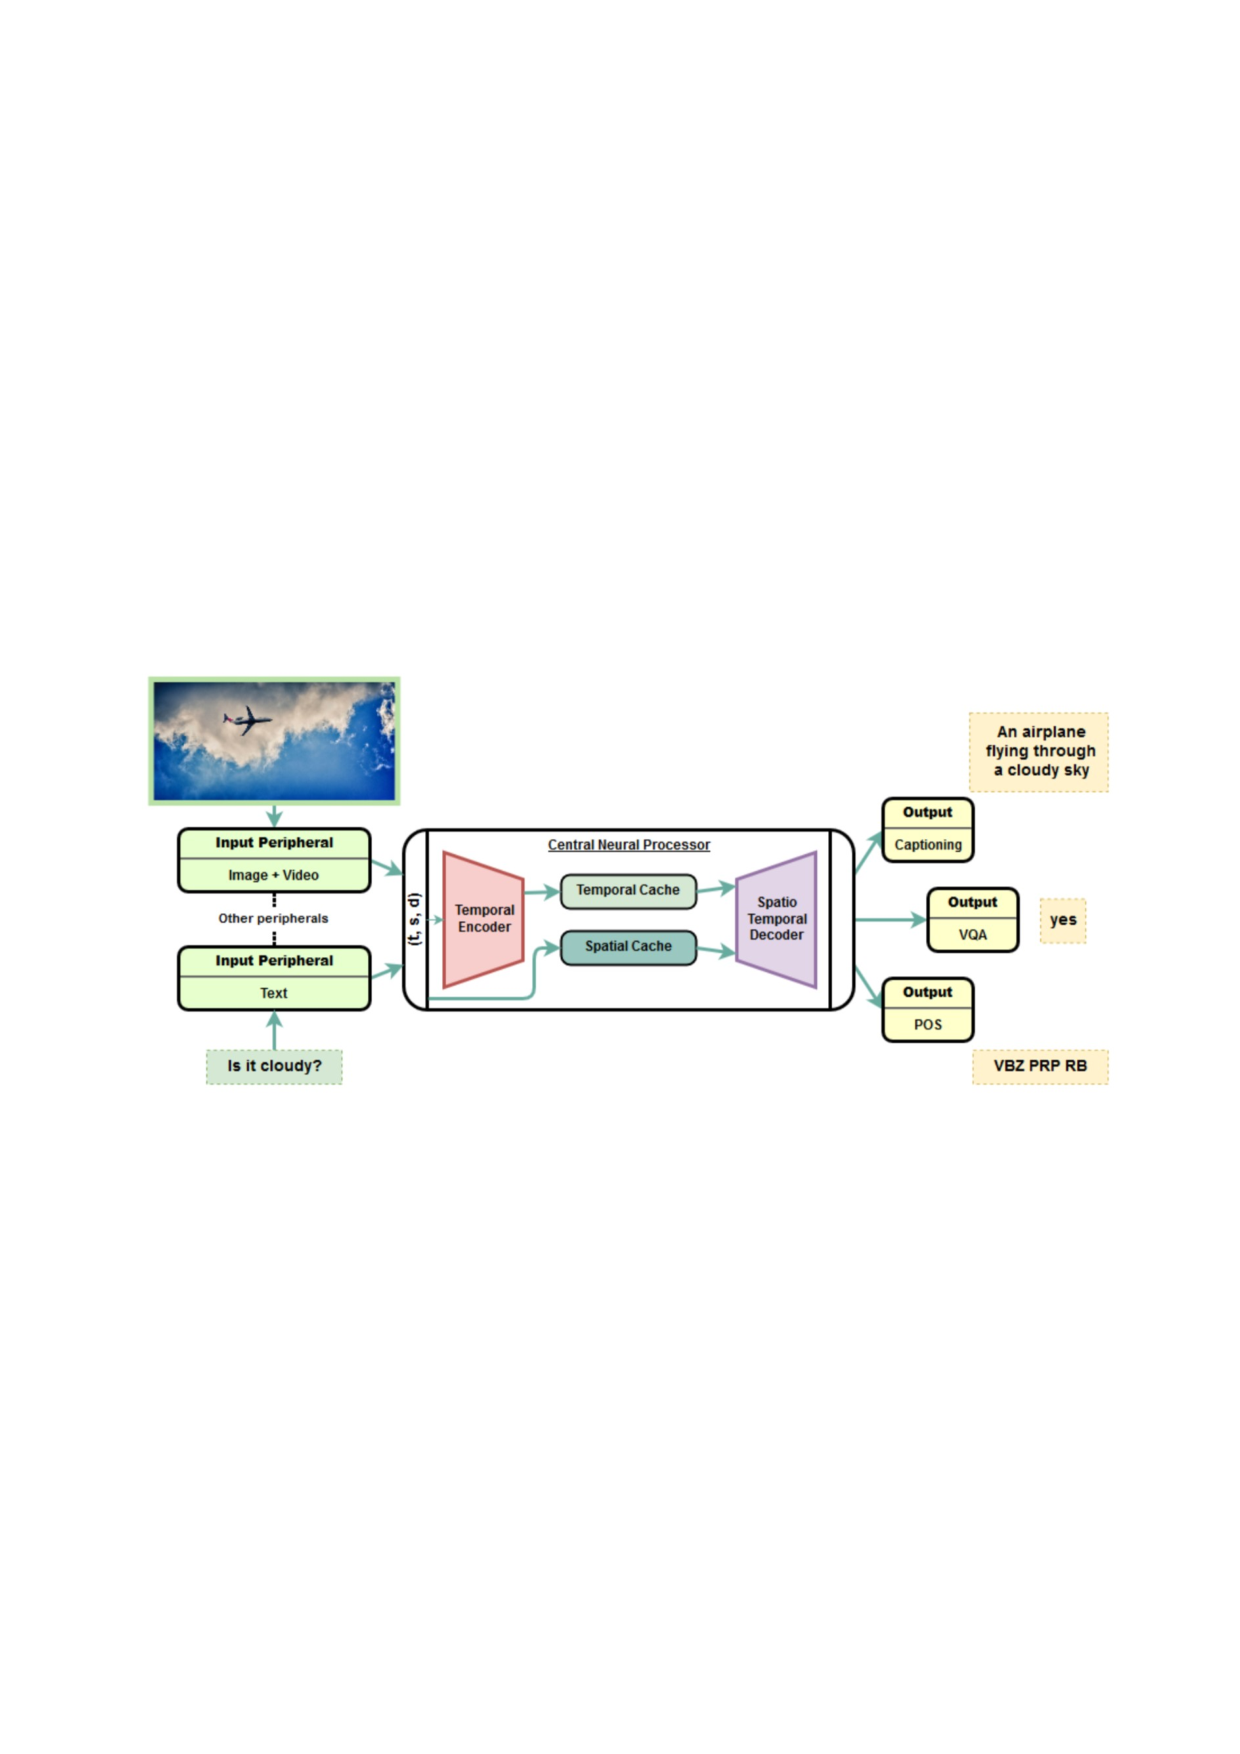
\includegraphics[width=0.7\textwidth]{OmniNet.pdf} 
		\caption{OmniNet from (Pramanik et al., 2019) \cite{pramanik2019omninet} performing image captioning, visual question answering and POS tagging at once.}
		\label{Fig.main4} 
	\end{figure*}



\subsection{Professional Machine Translation}

There are different technical terms between different research areas. It is obviously ridiculous that people who are not familiar with this field translate it, which is also the difference between a native speaker and non-native speaker. For example, in deep learning area, "transfer learning" not "migration learning", "object detection" not "target detection". Although their Chinese meaning is the same, if you translate them into the latter, you will be regarded as the people who unfamiliar with this field. Therefore, we introduce Professional Machine Translation, just like an expert with specific field knowledge to translate, make people feel particularly professional. In VMT, we can first through the Video Theme Inference task to determine the topic that is most relevant to this video and then extend the domain-specific knowledge of the topic. Therefore, it is possible to search within a specific range to improve the professionalism of the target sentence of the translation, and at the same time improve the efficiency of the translation. 











\bibliographystyle{unsrt}  
%\bibliography{references}  %%% Remove comment to use the external .bib file (using bibtex).
%%% and comment out the ``thebibliography'' section.


%%% Comment out this section when you \bibliography{references} is enabled.
% \begin{thebibliography}{1}


% \end{thebibliography}

\bibliography{references}


\end{document}
